% This is samplepaper.tex, a sample chapter demonstrating the
% LLNCS macro package for Springer Computer Science proceedings;
% Version 2.20 of 2017/10/04
%
\documentclass[runningheads]{llncs}
%
\usepackage{graphicx}
\usepackage{amsmath}
\usepackage{amsfonts}
\usepackage{float}
% Used for displaying a sample figure. If possible, figure files should
% be included in EPS format.
%
% If you use the hyperref package, please uncomment the following line
% to display URLs in blue roman font according to Springer's eBook style:
% \renewcommand\UrlFont{\color{blue}\rmfamily}

\hyphenation{wa-ter-mar-king}
\hyphenation{com-pressi-ve}
\hyphenation{mo-du-la-tion}
\hyphenation{images}
\hyphenation{Ho-we-ver}
\hyphenation{in-co-rrec-tly}

\begin{document}
%
\title{Dual watermarking for handwritten document image authentication, tamper detection and copyright protection for JPEG compression attacks}
%
%\titlerunning{Abbreviated paper title}
% If the paper title is too long for the running head, you can set
% an abbreviated paper title here
%
\author{Ernesto Avila-Domenech\inst{1}\orcidID{0000-0002-4797-289X} \and
Anier Soria-Lorente\inst{1}\orcidID{0000-0003-3488-3094} \and
Alberto Taboada-Crispi\inst{2}\orcidID{0000-0002-7797-1441}}
%
\authorrunning{E. Avila-Domenech et al.}
% First names are abbreviated in the running head.
% If there are more than two authors, 'et al.' is used.
%
\institute{Universidad de Granma, Carretera Central v{\'i}a Holgu{\'i}n Km $\frac{1}{2}$, Granma, Cuba \email{\{eadomenech, asorial1983\}@gmail.com}\\ \and
Universidad Central de Las Villas, Villa Clara, Cuba\\
\email{\{ataboada\}@uclv.edu.cu}}
%
\maketitle              % typeset the header of the contribution
%
\begin{abstract}
For authentication, tamper detection and copyright protection of handwritten document images, a dual watermarking algorithm that connects the robust watermarking algorithm based on Krawtchouk moments with a fragile watermarking algorithm based on MD5 hash function is presented. Hence, the robust watermarking algorithm is used to guarantee robustness by modifying frequency coefficients in Krawtchouk moments. Thus, this study proposes a fragile watermarking algorithm, which can perceive in time when the protected image is tampered. Experimental results show that the proposed algorithm can be used for copyright protection for JPEG compression attacks and tampering detection of this images.

\keywords{Handwritten  \and Image \and Watermarking.}
\end{abstract}
%
%
%
\section{Introduction}
The explosive growth of digital multimedia techniques, together with the rapid development of digital network communication has created a pressing demand for techniques that could be used for content authentication and copyright protection. Due to these needs, digital rights management (DRM) is gaining importance; it refers to a range of access control technologies used to limit or restrict the use of digital content. Digital watermarking is useful in DRM systems as it can hide information within the digital content like images, audio and video.

Watermarking technique is effectively applied to content authentication and copyright protection. In accordance with the desired robustness of the embedded watermark, digital watermarking techniques are divided into fragile watermarking and robust watermarking. The first one is designed to detect slight changes to the watermarked image with high probability and the second one is typically used for copyright protection, thus it is designed to resist attacks that attempt to remove or destroy the watermark without significantly degrading the visual quality of the watermarked image.

When users want to detect illegal tampering and protect the copyright at the same time, the single watermarking algorithm cannot meet the needs of users. Therefore, a dual watermarking algorithm is developed, as it can effectively combine the advantages and functions of the two watermarks \cite{wang2017dual}.

Numerous dual watermarking algorithms have been proposed. In \cite{mohanty1999dual}, a dual watermarking technique is presented which attempts to establish the owner’s right to the image and detect the intentional and unintentional tampering of the image. However, this early research is simply a combination of visible and invisible watermarking algorithms. In \cite{wang2017dual},  a dual watermarking algorithm that connects the robust watermarking algorithm based on singular value decomposition (SVD) with a fragile watermarking algorithm based on compressive sensing (CS) is presented. \cite{singh2018hybrid} uses cryptography and QR Code in combined approach of LSB and DCT, the authors combines the LSB and DCT approaches because LSB contains spatial domain property and DCT contains frequency domain property.

In \cite{shivani2017dual}, a gray scale logo used as copyright information of the owner is embedded imperceptibly into the singular values of the cover image in multiple locations, also performed pixel-wise authentication which fetched the advantage of accurate tamper localization in case of alterations. In \cite{liu2018blind}, a blind dual watermarking mechanism for digital color images is presented. The first watermark is embedded by using the discrete wavelet transform (DWT) in YCbCr color space, and it can be extracted blindly without access to the host image. However, fragile watermarking is based on an improved least significant bits (LSB) replacement approach in RGB components for image authentication. In \cite{singh2019robust}, a lifting wavelet transform (LWT) and discrete cosine transform (DCT) based robust watermarking approach for tele-health applications is presented. They are based on LWT, which requires less memory, it has reduced aliasing effects and distortion, fast and it is a good choice for low computational complexity than conventional DWT.

The aforementioned methods have been proposed for images in a general sense. Unlike these methods, our proposal is a dual watermark optimized for handwritten document images. 

The rest of the paper is organized as follow; Section 2 describes the proposed method including robust watermarking and fragile watermarking. Experimental results are given in Section 3 and Section 4 concludes the paper.

\section{Proposed method}
Dual watermarking implies embedding of fragile as well as robust watermarks into the same cover image. It facilitates integration of image authentication and copyright protection into the same scheme. First robust watermarking and then the fragile watermarking should be done because the fragile watermarking is sensitive to small changes. Unlike the fragile watermarking, the robust one resists changes caused by performing the fragile watermarking.
\begin{figure}
	\begin{center}
		\includegraphics[width=0.8\textwidth]{dual_watermarking.png}
		\caption{Dual watermarking.} \label{dual_watermarking}
	\end{center}
\end{figure}

\subsection{Robust watermarking}
The robust watermarking method proposed is similar to the one proposed in \cite{avila2018watermarking}. The difference consists of considering any binary image as a watermark. In the previous work only a QR code was considered as a watermark, so it was possible a restructuring of the extracted watermark making use of the characteristics related to the QR codes.
\begin{figure}
	\begin{center}
		\includegraphics[width=\textwidth]{WP.png}
	\end{center}
	\caption{Watermark embedding and extraction scheme. (Modified from \cite{avila2018watermarking})}
	\label{PIE}
\end{figure}

The following steps are taken during the embedding process:
\begin{enumerate}
	\item The binary watermark image is scrambled using Arnold transform \cite{Arnol'd:1987366}.
	\item The cover image is transformed from RGB to YCbCr color space, and the Y component, corresponding to the luminance information, is divided into small image blocks of $8\times 8$ pixels.
	\item A number of blocks equal to the number of bits to be inserted is selected from a given key.
	\item The Krawtchouk moments \cite{Yap2003} of the selected blocks are determined.
	\item Watermark bit is embedded in the selected block moments using Dither modulation \cite{chen2001quantization}. The values 19 and 128 are used as the coefficient and embedding strength values respectively. Watermarked blocks can be obtained. 
	\item The YCbCr to RGB color space is transformed to obtain RGB watermarked image.
\end{enumerate}

For watermark extraction:
\begin{enumerate}
	\item The watermarked image is transformed from the RGB to the YCbCr color space and the Y component is divided into $8\times 8$ pixels blocks.
	\item Some blocks are selected from which they will be extracted from the key used in the embedding process.
	\item The Krawtchouk moments of the selected blocks are determined.
	\item Scrambled watermark bits are obtained with the selected blocks moments using Dither modulations.
	\item Finally, a watermark is constructed with the scrambled bits using Arnold transform.
\end{enumerate}

\subsection{Fragile watermarking}
As we know, a hash function, such as MD5 or SHA-256, can be utilized to authenticate the data. If the hash value of original message is exactly equal to the re-calculated hash value of the received message, the received data can be regarded as integrated, otherwise as false.

For the process of embedding the following steps are performed each RGB component:
\begin{enumerate}
	\item The component is divided into $32\times 32$ non-overlapped blocks.
	\item 128 pixels of each block are selected by a given key.
	\item The least significant bit (LSB) of each selected pixel is assigned the value 0.
	\item The MD5 hash value of the modified block is generated as a watermark.
	\item The watermark is embedded into the LSB of the selected pixels and a watermarked block image is obtained.  
\end{enumerate}    

Detecting a fragile watermark water is the reverse process of embedding watermark, which is used to detect whether the watermarked image has been tampered and what the precise position of the tampered parts is. For this:
\begin{enumerate}
	\item The RGB image is divided into $32\times 32$ non-overlapped blocks.
	\item 128 pixels of each block are selected by a given key.
	\item Three binary series are formed from the LSBs of the selected pixels.
	\item The LSBs of each selected pixel are assigned the value 0.
	\item The MD5 hash value of the modified block is generated and compared with obtained series.
\end{enumerate}

\section{Experiments and Results}
The watermarking algorithm is evaluated through imperceptibility, tamper detection and robustness. Also, it is compared with the methods proposed in \cite{shivani2017dual} and \cite{liu2018blind}. This last method has the variable $k$ as a parameter, that corresponds to the strength of the watermark. A higher $k$ can increase the strength of the embedded watermark, but it makes the watermarked image easier to perceive. For this reason and to make a better comparison, we have taken four different $k$ values (0.2, 0.4, 0.8 and 1.0).   

We used two handwriten document image databases: Saint Gall \cite{fischer2011transcription} and Parzival \cite{fischer2009automatic} database. The first one contains manuscripts from the 9th century using Carolingian scripts by a single writer, while the Parzival is compiled from 13th century Gothic scripts \cite{pastor2016complete}.
 

\subsection{Imperceptibility}
We calculated the larger peak signal-to-noise ratio (PSNR) which compares the similarity between the original image $ I $, and the watermarked image $ I_w $. A higher PSNR indicates that the watermarked image more closely resembles the original image meaning that the watermark is more imperceptible.
\begin{figure}[H]
	\begin{center}
		\begin{tabular}{|c|c|}\hline
			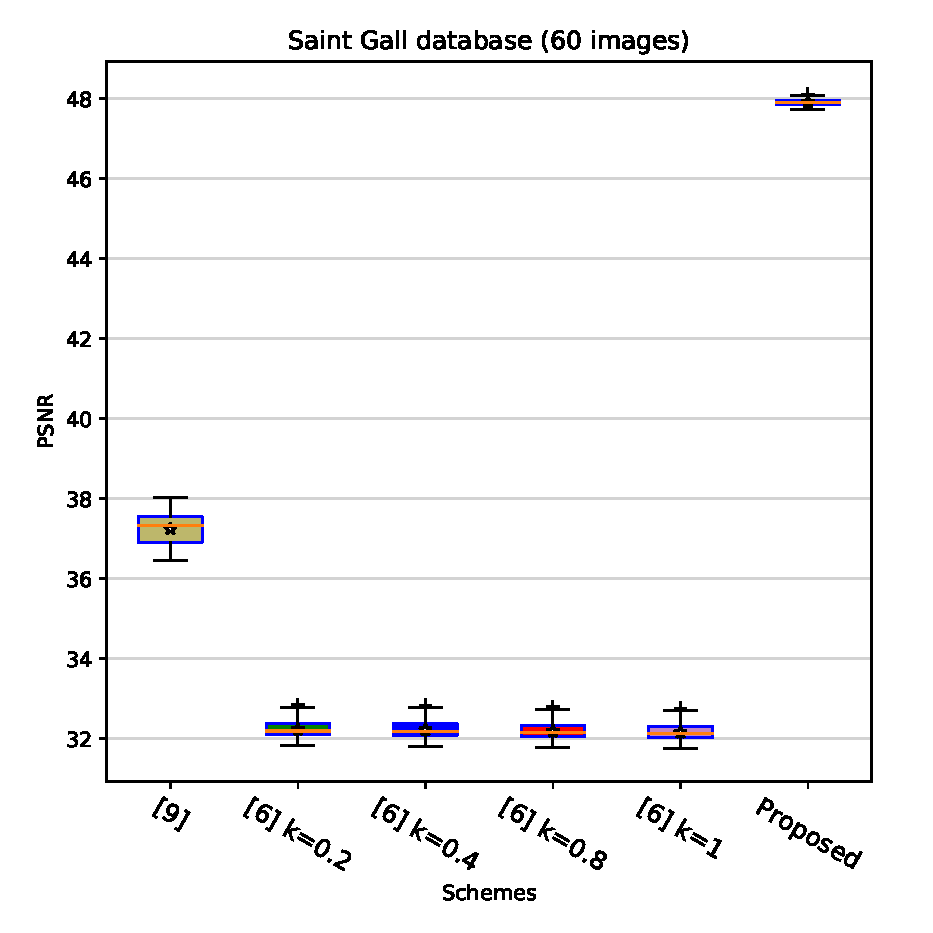
\includegraphics[width=0.5\textwidth]{PSNR_saintgall.eps}
			&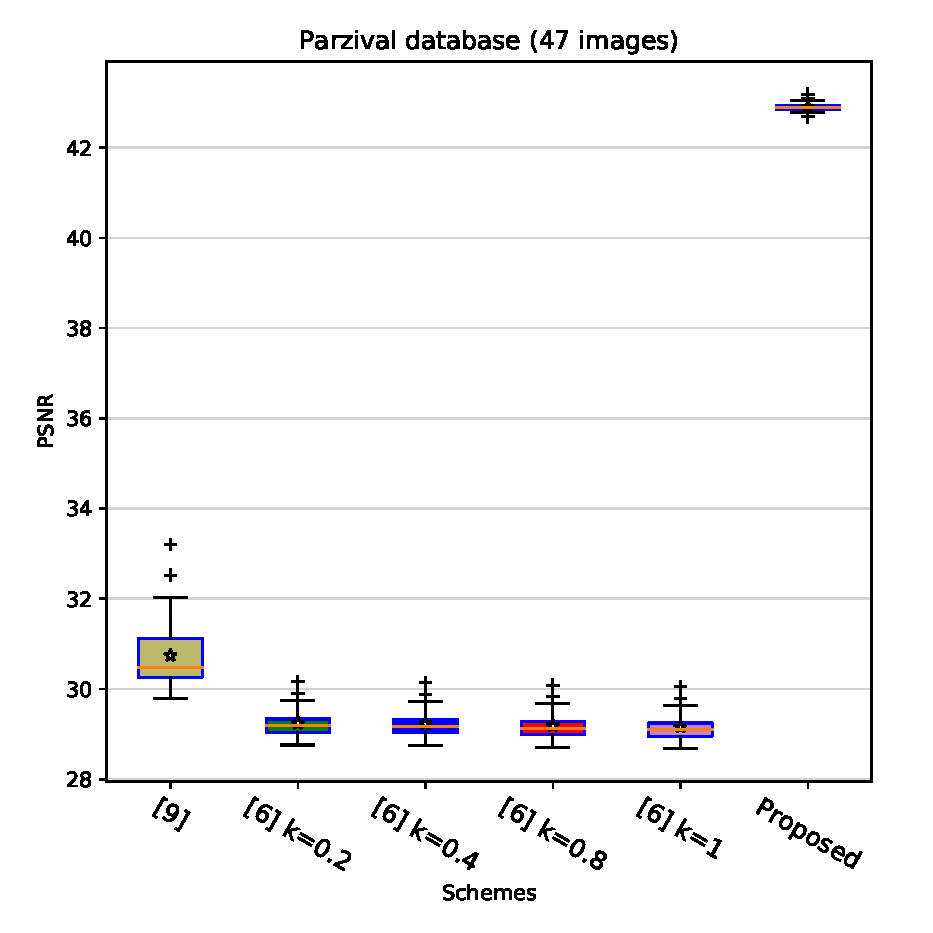
\includegraphics[width=0.5\textwidth]{PSNR_parzival.eps}\\\hline
		\end{tabular}
	\end{center}
	\caption{PSNR values for Saint Gall and Parzival database watermarked images.}
	\label{psnr}
\end{figure}
For both databases, the proposed method obtains higher values of PSNR compared to \cite{shivani2017dual} and \cite{liu2018blind} in its four variants (see Fig.~\ref{psnr}). Also, it can be noticed that \cite{shivani2017dual} provides improvements with respect to \cite{liu2018blind}. In addition, it is observable that by varying the parameter $k$, similar values of PSNR are contained.  
\begin{figure}
	\begin{center}
		\begin{tabular}{|c|c|}\hline
			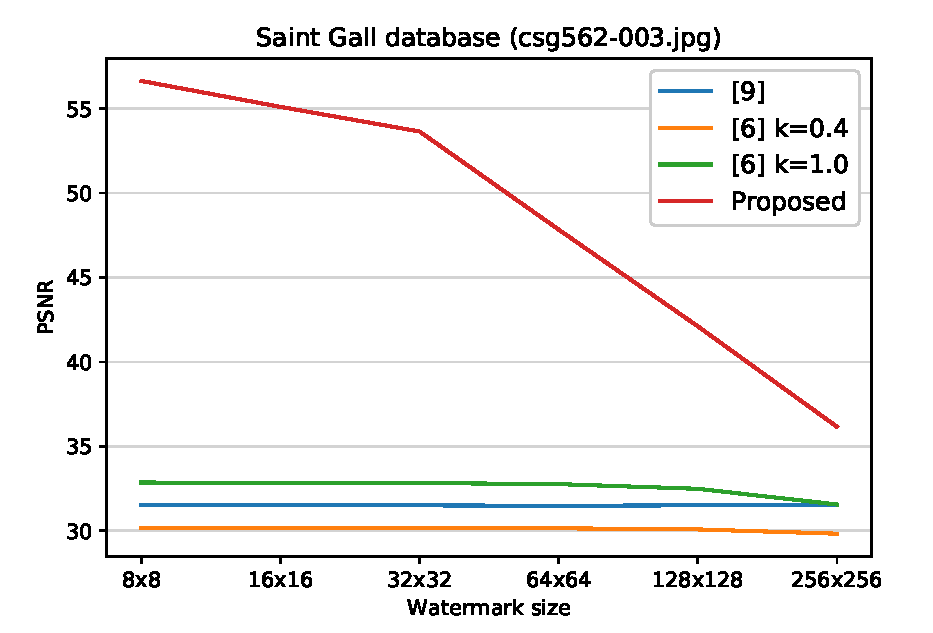
\includegraphics[width=0.5\textwidth]{PSNRwsizeSaintGall.eps}
			&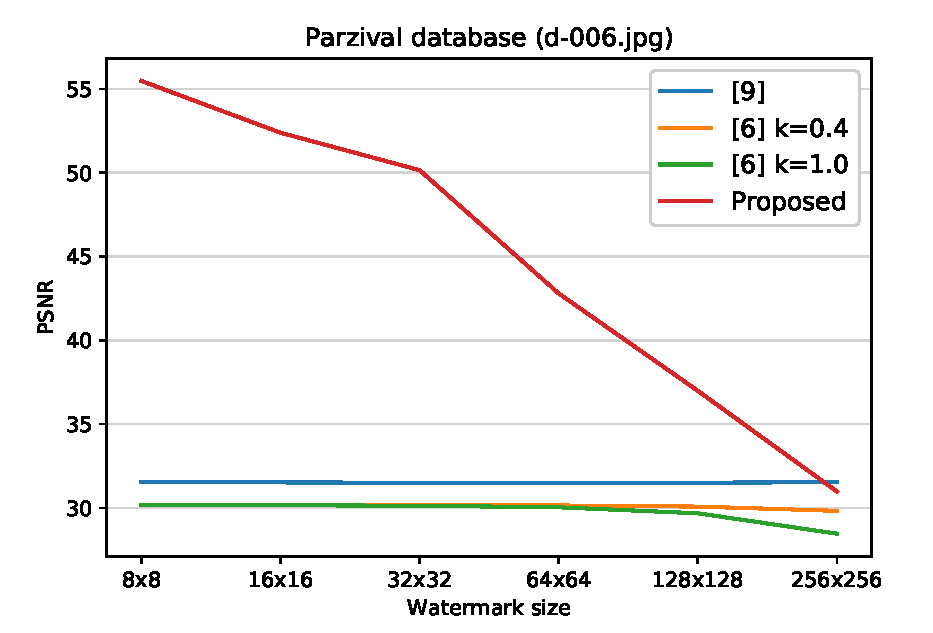
\includegraphics[width=0.5\textwidth]{PSNRwsizeParzival.eps}\\\hline
		\end{tabular}
	\end{center}
	\caption{PSNR behavior to mark the ``csg562-003.jpg'' image of Saint Gall database and ``d-006.jpg'' image of Perzival database with watermarks of different sizes.}
	\label{psnrwsize}
\end{figure}
\begin{figure}[H]
	\begin{center}
		\begin{tabular}{|c|c|c|c|}\hline
			\includegraphics[width=0.25\textwidth]{watermarked_Shivani2017.jpg}
			&\includegraphics[width=0.25\textwidth]{watermarked_Shivani2017_with_noise.jpg}
			&\includegraphics[width=0.25\textwidth]{tamper_zone.png}
			&\includegraphics[width=0.25\textwidth]{tamper_detection_Shivani2017.jpg}\\\hline
			\includegraphics[width=0.25\textwidth]{watermarked_Liu2018.jpg}
			&\includegraphics[width=0.25\textwidth]{watermarked_Liu2018_with_noise.jpg}
			&\includegraphics[width=0.25\textwidth]{tamper_zone.png}
			&\includegraphics[width=0.25\textwidth]{tamper_detection_Liu2018.jpg}\\\hline
			\includegraphics[width=0.25\textwidth]{watermarked_proposed.jpg}
			&\includegraphics[width=0.25\textwidth]{watermarked_proposed_with_noise.jpg}
			&\includegraphics[width=0.25\textwidth]{tamper_zone.png}
			&\includegraphics[width=0.25\textwidth]{tamper_detection_proposed.jpg}\\\hline
		\end{tabular}
	\end{center}
	\caption{Watermarked image, modified watermarked, tamper zone and tamper detection corresponding to \cite{shivani2017dual}, \cite{liu2018blind} and proposed scheme.}
	\label{tamper_detection}
\end{figure}

As a preliminary experiment, two images were taken, one from each database, and tests were performed to obtain the corresponding PSNR by varying the size of the watermark. For this case, the dimensions $8\times 8$, $16\times 16$, $32\times 32$, $64\times 64$, $128\times 128$ and $256\times 256$ pixels were taken as a watermark. As shown in Fig.~\ref{psnrwsize} the proposed method obtains better imperceptibility values for the first five dimensions, only in the sixth is it slightly exceeded by \cite{shivani2017dual}.

\subsection{Tamper detection}
Tamper area detection capability is evaluated, by modifying the contents of images. We developed our proposed fragile watermarking particularly for integrity images and locating tampered areas. Fig.~\ref{tamper_detection} shows the modified watermarked image by text addition, word substitution, underline words, content removal, and their corresponding tamper detection results.

The results obtained by \cite{shivani2017dual} are acceptable. Of the possible modifications, there is a 50\% probability that $\left( \sum_{m=1}^{5}XOR\right)\,  mod.\, 2$ is the same as the watermark bit. Likewise, both the \cite{liu2018blind} method and the proposed one detect the modifications made in an acceptable way.

\subsection{Robustness}
The robustness is measured as the bit error rate (BER) corresponding to incorrectly formed binary values of the watermark image.
\begin{figure}[H]
	\begin{center}
		\begin{tabular}{|c|c|}\hline
			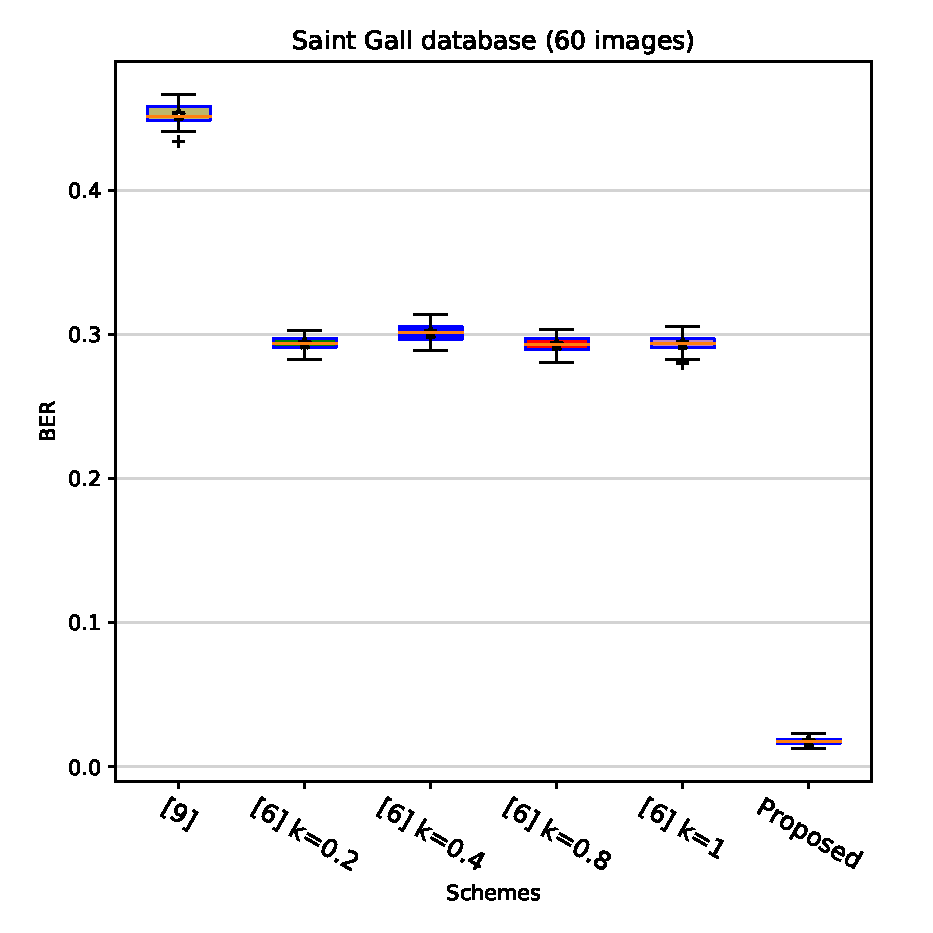
\includegraphics[width=0.5\textwidth]{BER75SaintGall.eps}
			&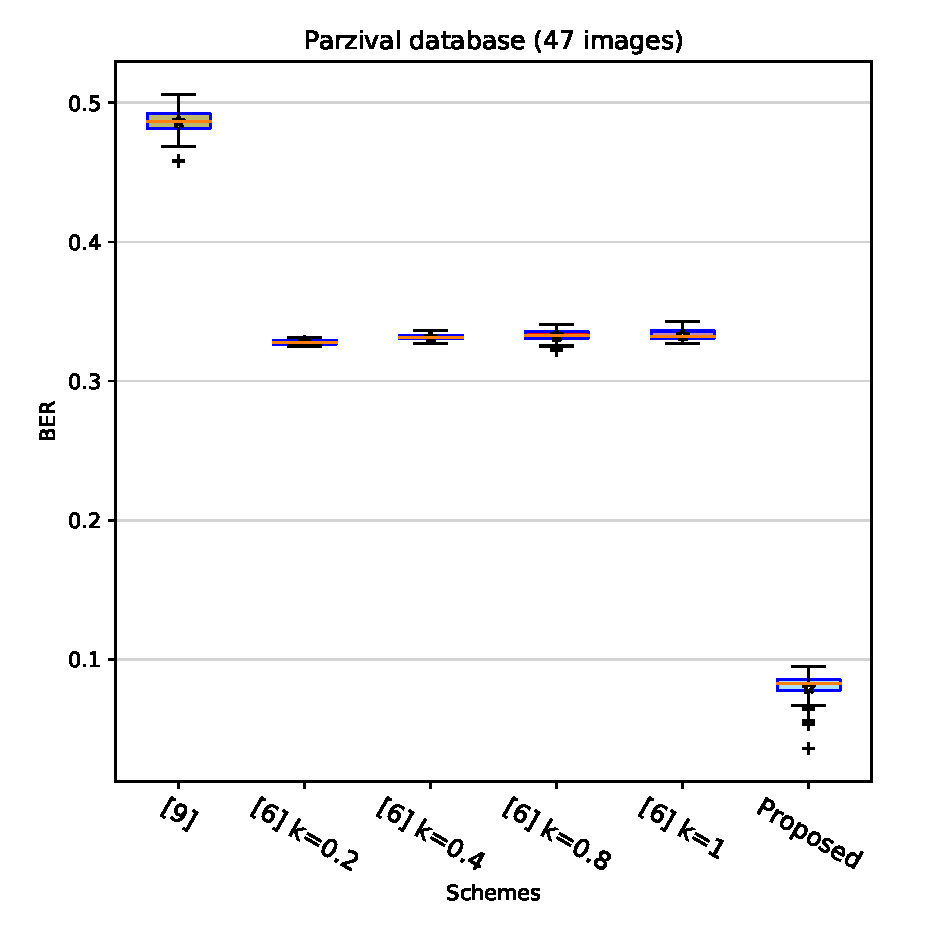
\includegraphics[width=0.5\textwidth]{BER75Parzival.eps}\\\hline
		\end{tabular}
	\end{center}
	\caption{BER values for watermarked images with JPEG compression (QF=75\%).}
	\label{ber75}
\end{figure}
The main contributions of this paper are of twofold. First is the obtaining of better values of imperceptibility, and the second is the remarkable improvement in the strength when JPEG compression attacks at 75\%, 50\% and 25\% are applied (see Figs. \ref{ber75}-\ref{ber25}). Similar to the PSNR, a preliminary experiment, using the same two images, was performed to obtain the corresponding BER by varying the size of the watermark.
\begin{figure}[H]
	\begin{center}
		\begin{tabular}{|c|c|}\hline
			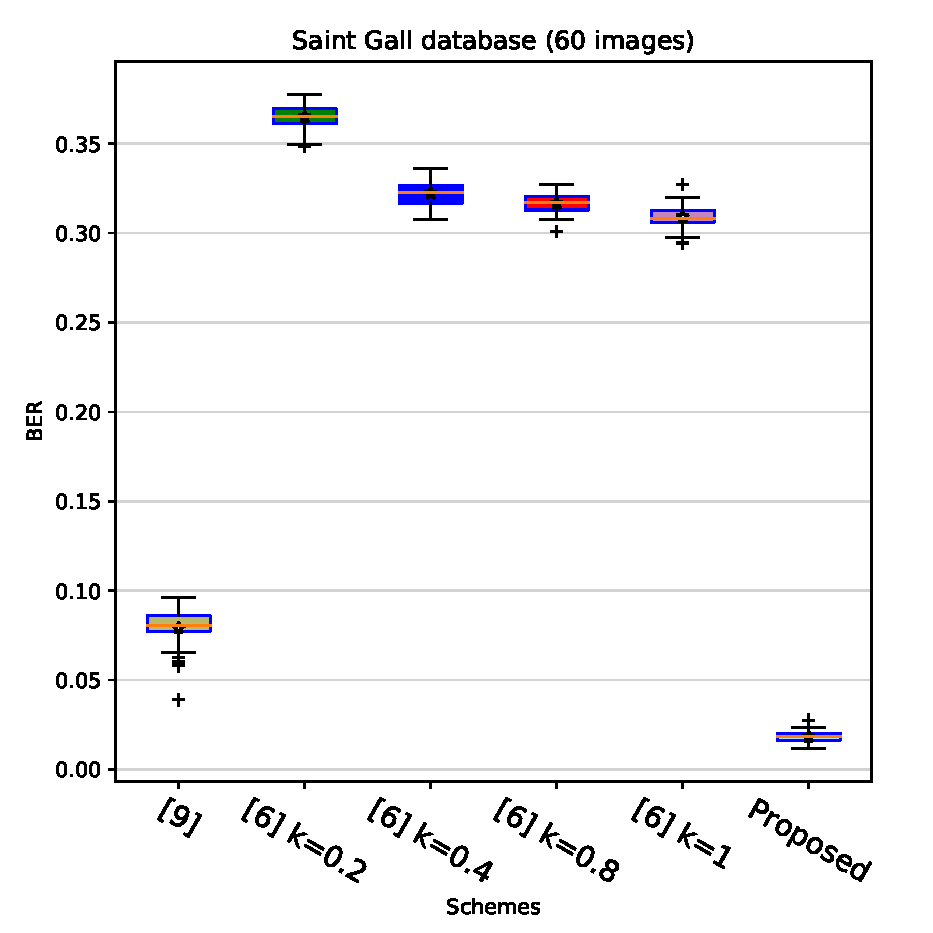
\includegraphics[width=0.5\textwidth]{BER50SaintGall.eps}
			&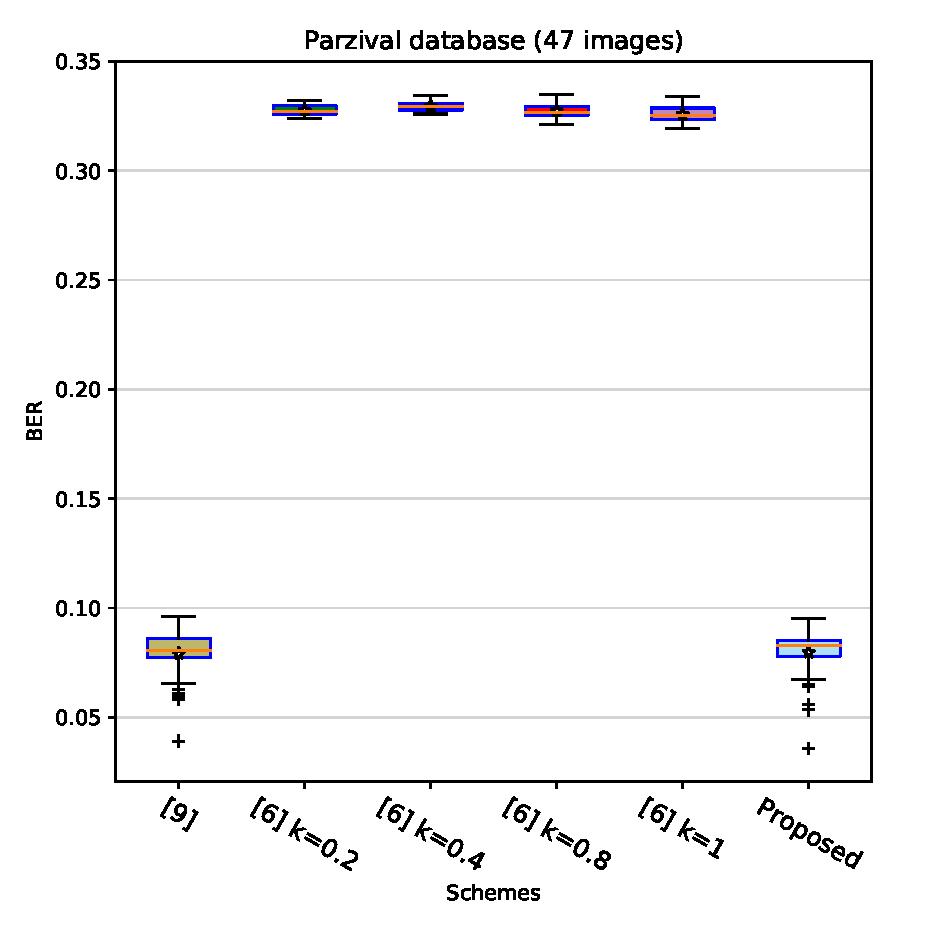
\includegraphics[width=0.5\textwidth]{BER50Parzival.eps}\\\hline
		\end{tabular}
	\end{center}
	\caption{BER values for watermarked images with JPEG compression (QF=50\%).}
	\label{ber50}
\end{figure}
\begin{figure}[H]
	\begin{center}
		\begin{tabular}{|c|c|}\hline
			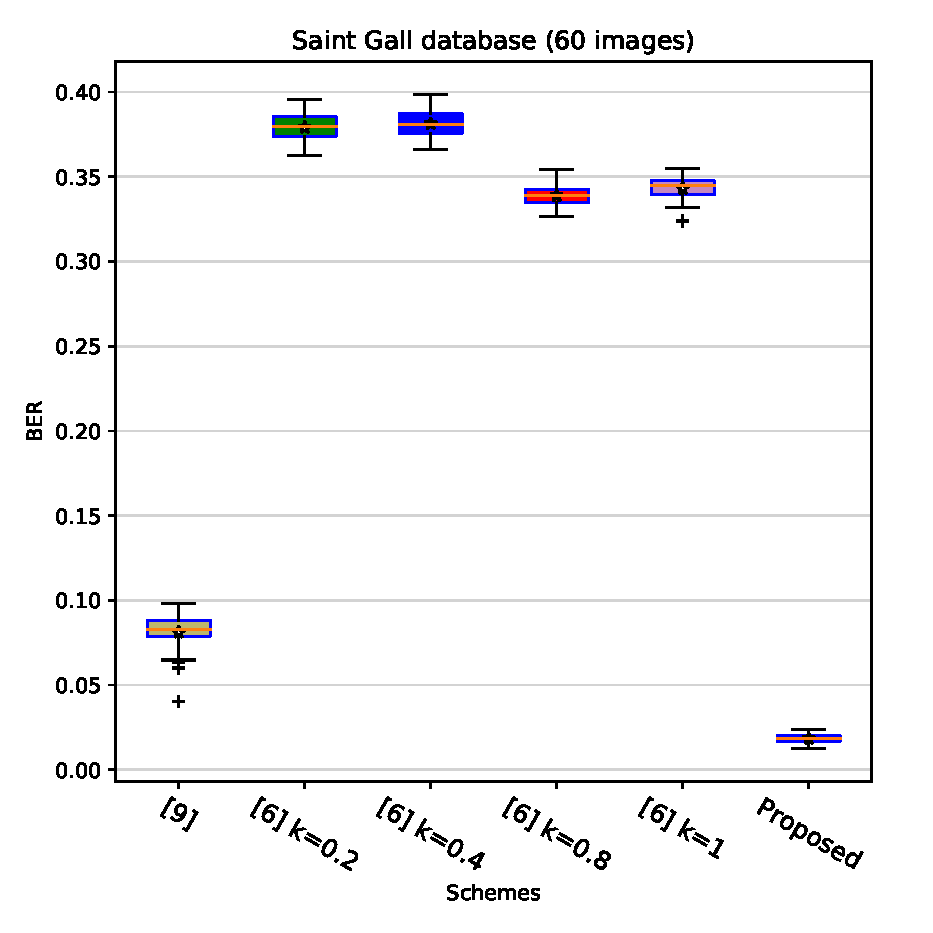
\includegraphics[width=0.5\textwidth]{BER25SaintGall.eps}
			&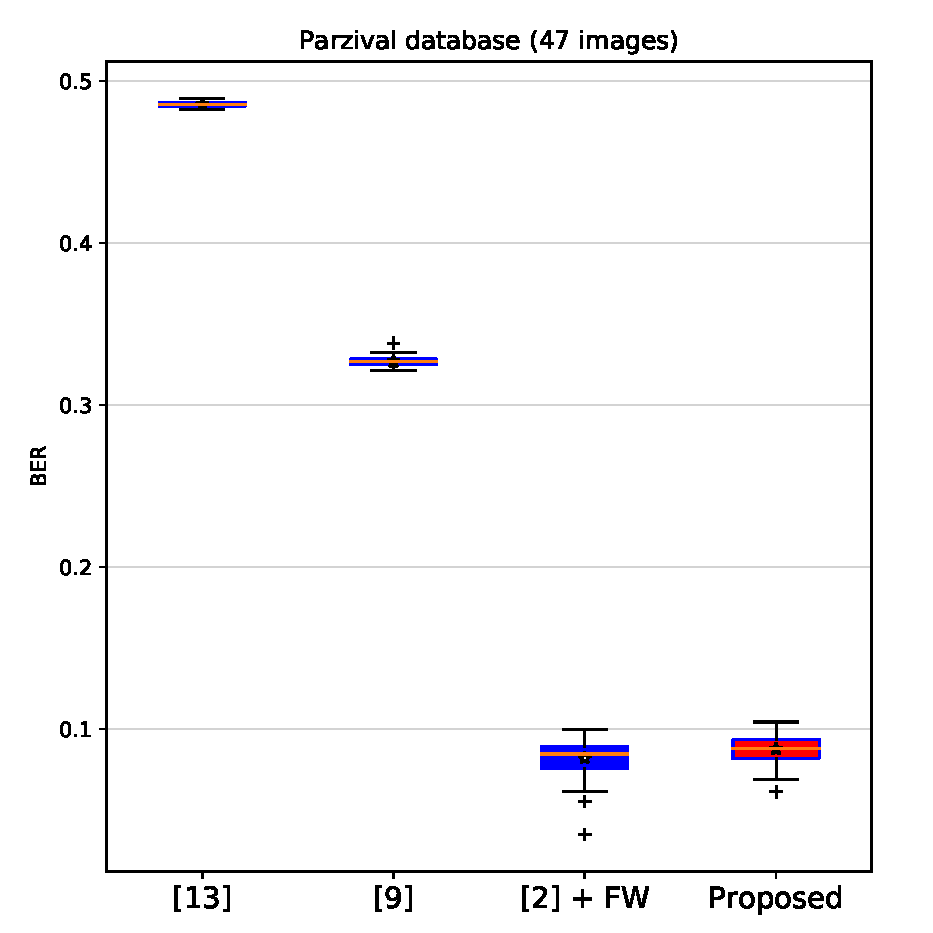
\includegraphics[width=0.5\textwidth]{BER25Parzival.eps}\\\hline
		\end{tabular}
	\end{center}
	\caption{BER values for watermarked images with JPEG compression (QF=25\%).}
	\label{ber25}
\end{figure} 

\begin{figure}
	\begin{center}
		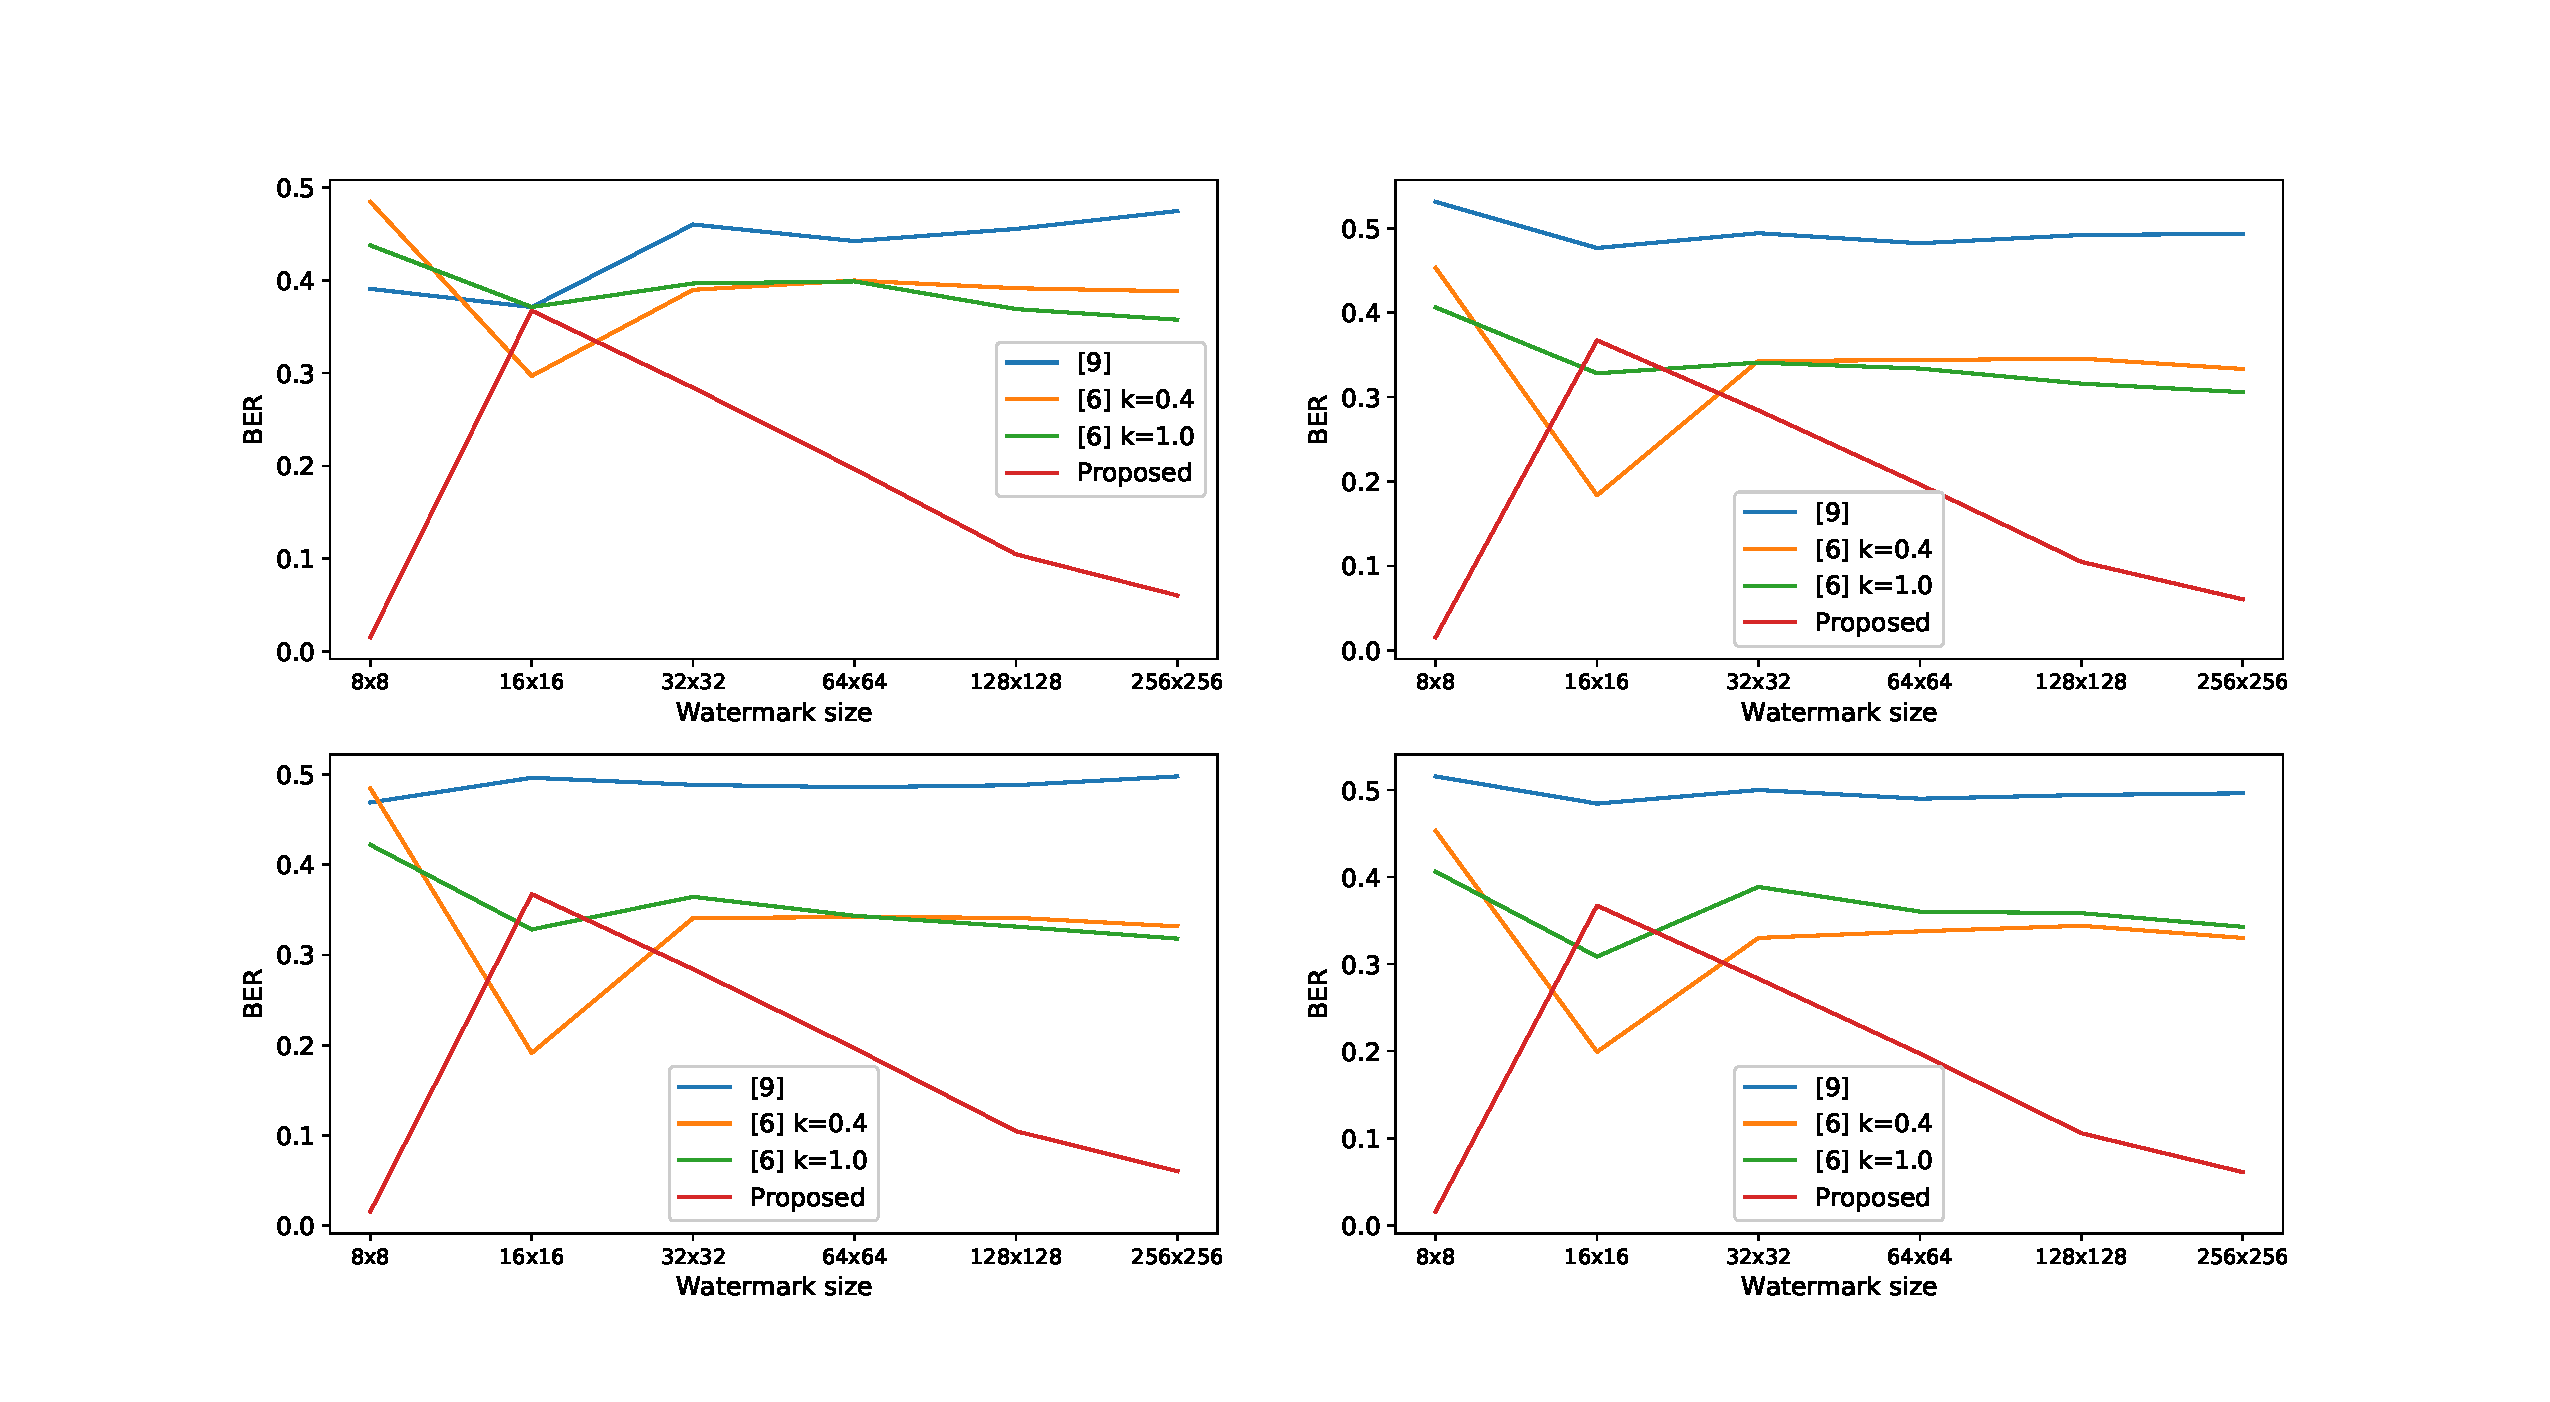
\includegraphics[width=1.1\textwidth]{BERwsizeSaintGall.eps}
		\caption{BER behavior to mark the image ``csg562-003.jpg'' of Saint Gall database with watermarks of different sizes when no attack is applied, a JPEG compression is performed with QF = 75\%, 50\% and 25\% respectively.} \label{berwsizeSaintGall}
	\end{center}
\end{figure}

\begin{figure}
	\begin{center}
		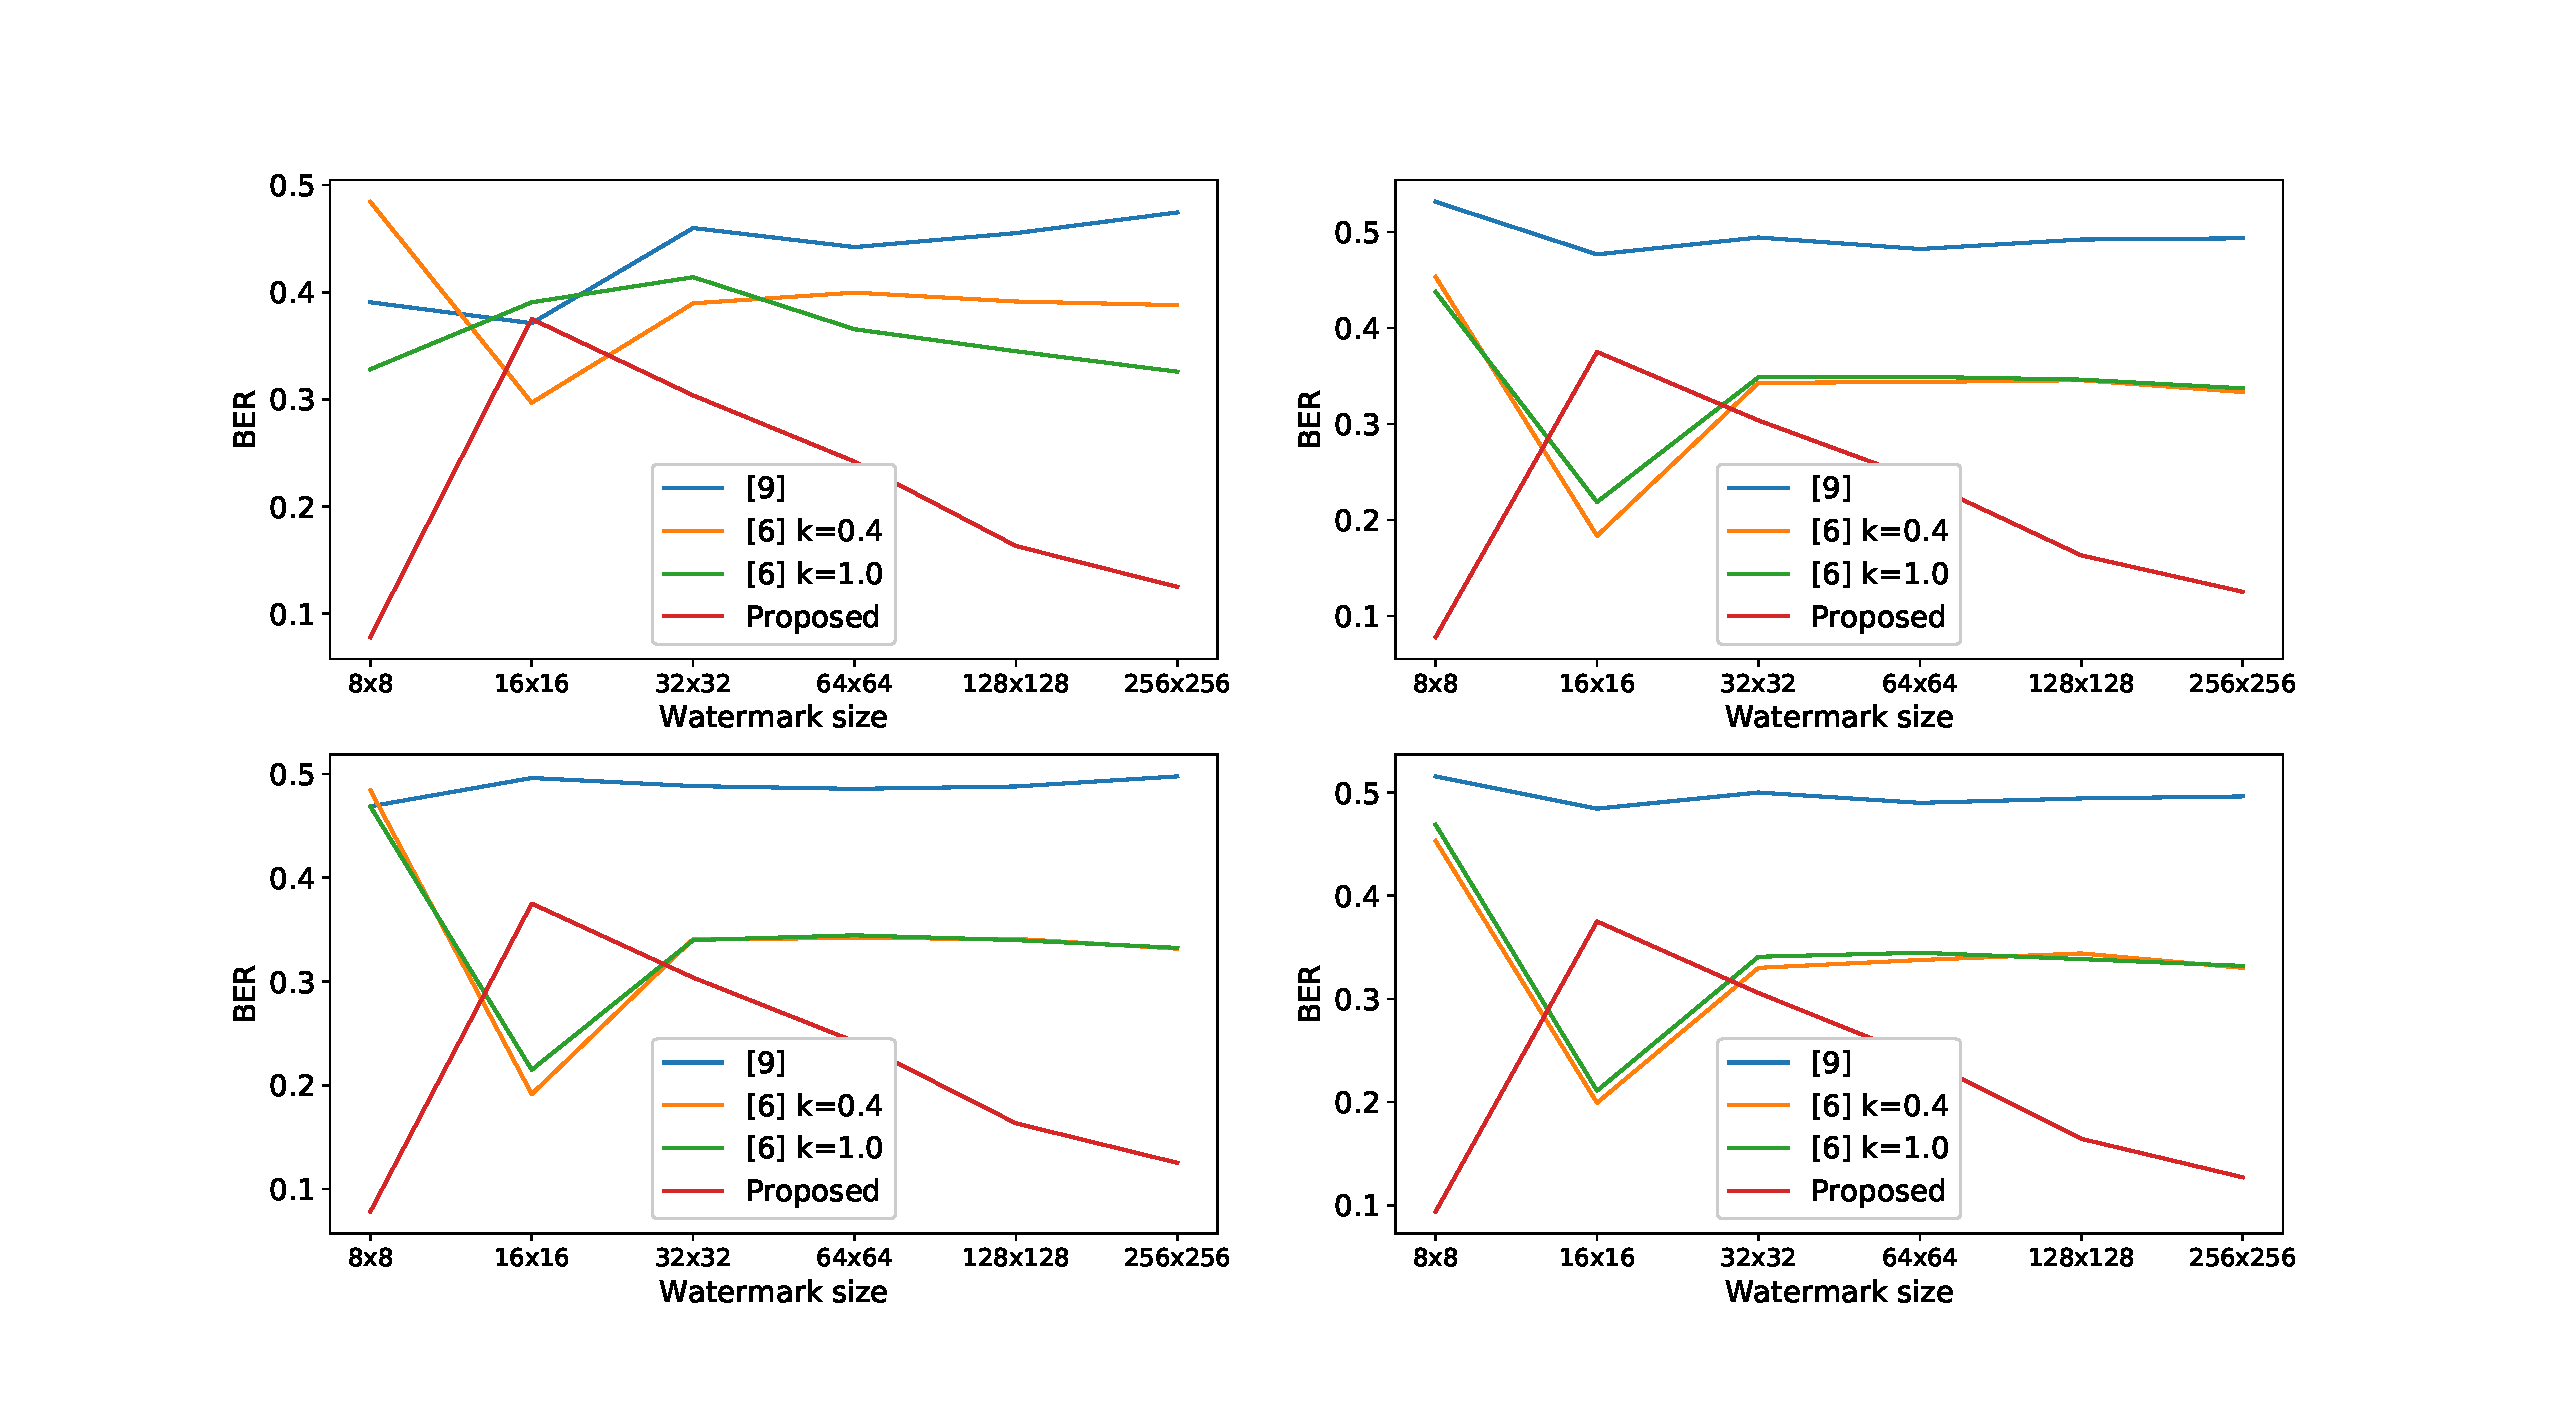
\includegraphics[width=1.1\textwidth]{BERwsizeParzival.eps}
		\caption{BER behavior to mark the image ``d-006.jpg'' of the Parzival database with watermarks of different sizes when no attack is applied, a JPEG compression is performed with QF = 75\%, 50\% and 25\% respectively.} \label{berwsizeParzival}
	\end{center}
\end{figure}

\section{Conclusions}
In this paper, a dual watermarking technique based on Krawtchouk moments and MD5 hash function was implemented. The experimental results show that our scheme is robust to JPEG compression attacks. In addition, the values corresponding to the PSNR were improved compared to previously presented papers.
%
% ---- Bibliography ----
%
% BibTeX users should specify bibliography style 'splncs04'.
% References will then be sorted and formatted in the correct style.
%
\bibliographystyle{splncs04}
\bibliography{mybibliography}
%
\end{document}
